\documentclass{standalone}
\usepackage{tikz}
\usetikzlibrary{positioning}
\usetikzlibrary{fit}

\begin{document}

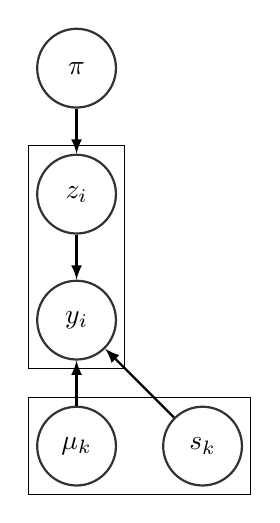
\begin{tikzpicture}
  \tikzstyle{random}=[circle, minimum size = 10mm, thick, draw = black!80, node distance = 16mm]
  \tikzstyle{connect}=[-latex, thick]
  \tikzstyle{plate}=[rectangle, draw = black!100]

  \node[random] (p) { $\pi$ };
  \node[random] (z) [below of = p] { $z_{i}$ };
  \node[random] (y) [below of = z] { $y_{i}$ };
  \node[random] (mu) [below of = y] { $\mu_{k}$ };
  \node[random] (s) [right of = mu] { $s_{k}$ };

  \path (p) edge [connect] (z)
        (z) edge [connect] (y);

  \path (mu) edge [connect] (y);

  \path (s) edge [connect] (y);

  \node[plate, inner sep = 1.0mm, fit = (z) (y)] { };
  \node[plate, inner sep = 1.0mm, fit = (mu) (s)] { };

\end{tikzpicture}

\end{document}
